\documentclass[]{article}

% use to waste space:
% \documentclass[12pt,a4paper]{article}

% if you have this style and like it.
%\documentclass{acmsiggraph}
%\documentclass[review]{acmsiggraph}      % review
%\documentclass[widereview]{acmsiggraph}  % wide-spaced review
%\documentclass[preprint]{acmsiggraph}    % preprint

% define a \comment{this is a comment which can have linebreaks in it}
\newcommand{\comment}[1]{}
% \newcommand{\todo}[1]{\marginpar{\bf{#1}}}
\newcommand{\todo}[1]{{\color{red}\bf{TODO: #1}}}

%\usepackage{mathptmx} % this fucked up mathcal H for H divergence
\usepackage[pdftex]{graphicx}
\usepackage[pdftex]{color}
\definecolor{rot}{RGB}{165,30,55} %rote Farbe
\graphicspath{{./images/}}
\usepackage{parskip}
\usepackage{amsmath, amssymb}
\usepackage{dsfont}
% \usepackage{pxfonts}


%\usepackage[T1]{fontenc}
%\usepackage{textcomp}

% comment these two lines out if you don't want minion/myriad fonts.
% \usepackage[minionint,mathlf]{MinionPro}
% \renewcommand{\sfdefault}{Myriad-LF}
%\usepackage{Myriad}
% no page number on float pages, fixes problems with overlarge diagrams.
\usepackage{fancyhdr}

\pagestyle{fancy}
%\lhead{}
%\chead{}
%\rhead{}
%\lfoot{}
\fancyhf{}
\fancyhead[EL]{\nouppercase{\leftmark}}
\fancyhead[OR]{\nouppercase{\rightmark}}
\cfoot{}
%\fancyfoot[EL]{\iffloatpage{}{\thepage}}
%\fancyfoot[OR]{\iffloatpage{}{\thepage}}
\fancyfoot[EL]{\thepage}
\fancyfoot[OR]{\thepage}
\renewcommand{\headrulewidth}{0pt}
\renewcommand{\footrulewidth}{0pt}

%\usepackage{natbib}		% textual referencing
%\usepackage[numbers,super]{natbib}	% nice superscripts
%\bibliographystyle{chicago}	% shitty
\bibliographystyle{alpha}	% abbr names and year in \cite
%\bibliographystyle{agsm}	% australian, need natbib
%\bibliographystyle{kluwer}	% need natbib
%\bibliographystyle{apalike}	% lengthly
%\bibliographystyle{abbrv}	% minimal?

% use for german line breaking:
%\usepackage[ngerman]{babel}
%\usepackage[T1]{fontenc}
\usepackage[utf8x]{inputenc}

% avoid us-style text color destruction:
\frenchspacing
\usepackage{microtype}

% have a nice framebox with border directly around the image:
\fboxsep 0pt
\newcommand{\fimg}[2]{\fbox{\includegraphics[width=#1]{#2}}}

\usepackage{theorem}
\theorembodyfont{\upshape}
\newtheorem{definition}{Definition}

\usepackage{listings}
\lstset{numbers=left, numberstyle=\tiny, basicstyle=\tiny, language=C++}
\usepackage[boxruled]{algorithm2e}
%\usepackage{hyperref}
\usepackage{url}
\usepackage{subfig}

\def\code#1{{\tt{#1}}}
%opening
\title{}
\author{}

\begin{document}
	
	\maketitle

This chapter is just a collection of notes on papers on \textbf{Domain Adaptation}.


\section{Domain Adaptation for Structured Output via Discriminative Patch Representation}

see \cite{Tsai2019DomainAF}

\subsection{Abstract}
\begin{itemize}
	\item labeling data is expensive
	\item therefore propose domain adaptation method to adapt labeled source data to unlabeled target domain (e.g. GTA5 (playing for data) to city-scapes)
	\item learn discriminative feature representations of patches based on label histograms in the source domain, through construction of clustered space
	\item then use adversarial learning sscheme to push feature representations in target patches to the closer distributions in source ones
	\item can integrate a global alignment process with this patch-level alignment and achieve state-of-the-art performance on semantic segmentation
	\item extensive ablation studies on numerous benchmark datasets with various settings (e.g. synth-to-real, cross-city)
\end{itemize}

\subsection{Introduction}

\begin{itemize}
	\item pixel-level annotation of ground truth expensive. e.g. road-scene iamges of different cities may have various appearance distributions, differences over time and weather
	\item existing state-of-the-art methods use feature-level or output space adaptation, exploiut global distribution alignment, such as spatial layout, but these might differ significantly between two domains due to differences in camera poses or field of view
	\item authours instead match patches that are more likely to be shared across domains regardless of where they are located
	\item consider label histograms as a factor (Kulkarni et al., 2015; Odena et al., 2017) and learn discriminative representations for patches to relax high-variation problem among them
	\item use this to better align patches between source and target domains
	\item utilize two adversarial modules to align global/patch-level distributions
	\item global one based on output space adaptation (Tsai et al. 2018)
	\item take source domain labels and extract label histogram as a patch-level representation
	\item then apply K-means clustering to group extracted patch representations into $K$ clusters \todo{read this part again for better understanding (page 2)}
\end{itemize}

\subsection{domain adaptation for structured output}

\begin{itemize}
	\item given source and target images $I_s,I_t \in \mathbb{R}^{H \times W \times 3}$ and source labels $Y_s$, the goal is to align predicted output distribution $O_t$ of target data with source distribution $O_s$
	\item use loss function for supervised learning on source data to predict the structured output, adversarial loss is adopted to align the global distribution
	\item further incorporate classification loss in a clustered space to learn patch-level discriminative representations $F_s$ from source output distribution $O_s$. For target data another adversarial loss is used to align patch-level distributions between $F_s$ and $F_t$, where the goal is to push $F_t$ to be closer to distributon of $F_s$.
	\item objective function :
	\begin{align}
		\mathcal{L}_{\text{total}}(I_s, I_t, Y_s, \Gamma(Y_s)) = \mathcal{L}_s + \lambda_d \mathcal{L}_d + \lambda_{\text{adv}}^g \mathcal{L}_{\text{adv}}^g + \lambda_{\text{adv}}^l  \mathcal{L}_{\text{adv}}^l
	\end{align}
	where $\mathcal{L}_s$ and $\mathcal{L}_d$ are supervised loss function for learning structured prediction and discriminative representation on source data. $\Gamma$ denotes clustering process on ground truth label distribution. $\mathcal{L}_{\text{adv}}^g, \mathcal{L}_{\text{adv}}^l$ denote global and patch-level adversarial loss. $\lambda$'s are weights for the different loss function
	\item $\mathcal{L}_s$ can be optimized by fully-convolutional network $\mathbf{G}$ that predicts the structured output with the loss summed over the spatial map indexed with $h,w$ and number of categories $C$:
	\begin{align}
		\mathcal{L}_s(I_s, Y_s;\mathbf{G}) = - \sum_{h,w}\sum_{c \in C} Y_s^{(h,w,c)}\log(O_s^{(h,w,c)})
	\end{align}
	where $O_s = \mathbf{G}(I_s) \in (0,1)$ is the predicted output distribution through softmax function and is up-sampled to the size of the input image.
	\item with discriminator $\mathbf{D}_g$:
	\begin{align}
		\mathcal{L}_{\text{adv}}^g(I_s, I_t; \mathbf{G}, \mathbf{D}_g) = \sum_{h,w}\mathbb{E}[\log\mathbf{D}_g(O_s)^{(h,w,1)}] + \mathbb{E}[\log(1- \mathbf{D}_g(O_t)^{(h,w,1)})]
	\end{align}
	\item optimize following min-max problem with inputs dropped for simplicity:
	\begin{align}
		\underset{\mathbf{G}}{\min} ~ \underset{\mathbf{D}_g}{\max} \mathcal{L}_s(\mathbf{G}) + \lambda_{\text{adv}}^g \mathcal{L}_{\text{adv}}^g(\mathbf{G}, \mathbf{D}_g)
	\end{align}
	\item label histograms for patches: first randomly sample patches from source images, using a 2-by-2 grid on patches to extract spatial label histograms, and concatenate them into a vector, each histogram is a $2 \cdot 2 \cdot C$ dimensional vector. Second apply K-means clustering on these histograms, whereby the label for any patch can be assigned as the cluster center with the closest distance on the histogram
	\item add classification module $\mathbf{H}$ after the predicted output $O_s$, to simulate the procedure of constructin the label histogram and learn a discriminative representation\\
	learned representation: $F_s = \mathbf{H}(\mathbf{G}(I_s)) \in (0,1)^{U \times V \times K}$ (softmax function, $K$ is number of clusters)
	\item learning process to construct clustered space formulated as cross-entropy loss:
	\begin{align}
		\mathcal{L}_d(I_s, \Gamma(Y_s); \mathbf{G}, \mathbf{H}) = - \sum_{u,v} \sum_{k\in K} \Gamma(Y_s)^{(u,v,k)}\log(F_s^{(u,v,k)})
	\end{align}
	\item goal is now to align patches regardless of where they are located in the image (without spatial and neighborhood support)
	\item reshape $F$ by concatenating the $K$-dimensional vectors along the spatial map, results in $U \cdot V$ independent data points
	\item this reshaped data is denoted as $\hat{F}$, adversarial objective:
	\begin{align}
		\mathcal{L}_{\text{adv}}^l(I_s, I_t; \mathbf{G}, \mathbf{H}, \mathbf{D}_l) = \sum_{u,v}\mathbb{E}[\log \mathbf{D}_l(\hat{F}_s)^{(u,v,1)}] + \mathbb{E} [\log(1- \mathbf{D}_l(\hat{F}_t)^{(u,v,1)})]
	\end{align}
	where $\mathbf{D}_l$ is the discriminator to classify whether the feature representation $\hat{F}$ is from source or target domain
	\item integrate (3.5) and (3.6) into min-max problem in 3.4:
	\begin{align}
		\underset{\mathbf{G}, \mathbf{H}}{\min} ~ \underset{\mathbf{D}_g, \mathbf{D}_l}{\max} \mathcal{L}_s(\mathbf{G}) + \lambda_d \mathcal{L}_d (\mathbf{G}, \mathbf{H}) + \lambda_{\text{adv}}^g, \mathcal{L}_{\text{adv}}^g(\mathbf{G}, \mathbf{D}_g) + \lambda_{\text{adv}}^l \mathcal{L}_{\text{adv}}^l(\mathbf{G}, \mathbf{H}, \mathbf{D}_l)
	\end{align} 
\end{itemize}



\section{Effective Use of Synthetic Data for Urban Scene Semantic Segmentation}

see \cite{DBLP:journals/corr/abs-1807-06132}

\begin{itemize}
	\item foreground and background classes are not affected the same way by domain shifts
	\item foreground classes should be treated in a detection based manner as their shape looks natural even though their texture in synthetic images is not photo-realistic
	\item drawback of deep neural networks is need for massive amount of training data
	\item training on synthetic only makes models perform bad in the real world
	\item domain adaptation methods improve this but still require large sets of real images
	\item model cannot be trained off-line on synthetic data and work well when deployed into a new, real-world environment
	\item observation: not all classes suffer from the same type and degree of perceptual differences
	\item background texture looks more realistic than foreground, nevertheless foreground object shape look natural
	\item therefore should be treated differently
	\item use semantic segmentation on background classes because of texture realism
	\item use object detectors for foreground classes
	\item main discrimination between fore and background objects is shape
	\item trained seperately a DeepLab and Mask R-CNN \todo{cite} for object detection, followed by binary segmentation and class prediction, on synthetic data
	\item compare mIoU on foreground classes of Cityscapes
	\item outperforms semantic segmentation model on every class except \textit{motorcycle}
	\item from this observation: model that combines foreground masks produced by Mask R-CNN with pixel-wise predictions of DeepLab semantic segmentation network
	\item outperforms state-of-the-art domain adaptation techniques and can be further improved by making use of unsupervised real images
	\item \textbf{VEIS} (Virtual Environment for Instance Segmentation) proposed aswell, based on Unity3D
	\item automatically annotates synthetic images with instance-level segmentation for foreground classes
	\item when used with the proposed detector-based approach this data allows to boost semantic segmentation performance
\end{itemize}

\subsection{related work}

\begin{itemize}
	\item domain adaptation generally aims to reduce the gap between the feature distributions of the two domains (synthetic, real)
\end{itemize}

\subsection{Method}

\begin{itemize}
	\item use VGG16-based DeepLab model for background classes (with large field of view and dilated convolution layers)
	\item train on GTA5 dataset (background classes look photo-realistic)
	\item cross-entropy loss between network's predictions and ground-truth pixel-wise annotations of the sythetic images
	\item trained on fore- and background classes but foreground predictions are mostly discarded by the proposed approach
	\item use standard Mask R-CNN (object detection, binary mask extraction together with object classification) \todo{look at citation}
	\item fuse fore- and background predictions
	\item sort predicted segments according to confidence score, if current segment candidate overlaps with previous segment, pixels are removed in the overlapping region
	\item this yields a semantic segmentation map that only contains foreground classes and has large number of holes where no foreground object was found. Every pixel that is not already assigned to foreground class takes the label with highest probability at that pixel location in the DeepLab result
	\item remember: NO real data used during training of this method
	\item to extend approach for unsupervised training on real images: tread predictions of their method as pseudo ground truth for the real images. assign pixels that ware predicted as foreground classes by DeepLab model to an \textit{ignore} label, so that they are not used for training. 
\end{itemize}

\subsection{Implementation Details}
\begin{itemize}
	\item DeepLab: SGD, learning rate starting at $25 \times 10^{-5}$ with decrease factor of 10 every 40k iterations, momentum of 0.9, weight decy of 0.0005, mini-batches of size 1. weights initialized with those of VGG-16 classifier, pre-trained on ImageNet, due to limited GPU memory high resolution images were downsampled by a factor of 2 for training
	\item Mask R-CNN: implementation provided by Detectron framework \todo{cite}, train an end-to-end Mask R-CNN model with $64 \times $ 4d ResNeXt-101-FPN backbone, pre-trained on ImageNet, on the synthetic VEIS dataset. mini-batch of size 1, train model for 200k iterations, starting learning rate of 0.001, reducing to 0.0001 after 100k iterations
\end{itemize}


\section{Exemplar Guided Unsupervised Image-to-Image Translation with Semantic Consistency}

see \cite{DBLP:journals/corr/abs-1805-11145}

\begin{itemize}
	\item EGSC-IT network conditions the translation process on an exemplar image in the target domain
	\item assumption: image comprises of a content component shared across domains, and style component specific to each domain
	\item under guidance of exemplar from target domain apply Adaptive Instance Normalization to the shared content component, which allows to transfer the style information of the target domain to the source domain
	\item introduce feature masks that provide coarse semantic guidance without requiring the use of any semantic labels to avoid semantic inconsistencies during translation
	\item image-to-image (I2I) translation: task of mapping an image from a source domain to a target domain (e.g. semantic maps to real images, grey-scale to color, low-resolution to high-res)
	\item other approaches assume one-to-one mapping (e.g. cycleGAN) and fail to capture multimodal nature of image distribution within the target domain (many-to-many mapping, e.g. diffferent color and style of shoes in sketch-to-image translation, different seasons in syn2real street view translation)
	\item assume an image is composed of two disentangled representations: domain-shared representation that models the content in the image, second domain-specific representation that contains the style information
	\item unclear which style (time-of-day/season) to pick during image translation process, Isola et al. 2017 and Zhu et al. 2017b \todo{cite} show that using random noise for this can lead to mode collapse issues
	\item instead the image translation process is conditioned on arbitrary image in the target domain (i.e. an exemplar)
	\item like this EGSC-IT is enabled for multimodal (i.e. many-to-many) image translations, but also allows for explicit control over translation process depending on the exemplars used as guidance
	\item use weight sharing architecture proposed in UNIT (Liu et al. 2017 \todo{cite}), but instead of single latent space shared by both domains, a two component one is used (domain-shared component that contains semantic information (objects' category, shape, spacial layout), domain-specific style component that contains style information (texture, color)
	\item adaptive instance normalization (AdaIN) (Huang \& Belongie 2017 \todo{cite}) is applied to the shared content component of the source domain image using AdaIN parameters computed from the target domaoin exemplar
	\item directly applying AdaIN to the feature maps of the shared content component would mix up all objects and scenes in the image, making the image translation prone to failure when a n image contains diverse objects and scenes, therefore semantic labels as an additional form of supervision is used \todo{cite works that do this}. 
	\item instead of using data with labor-intensive annotations use computed feature masks
	\item feature masks: approximately decoupling different semantic categories in an unsupervised way under guidance of perceptual loss and adversarial loss
\end{itemize}

\subsection{Method}
\begin{itemize}
	\item weight sharing: to map image pairs (one from source domain, other target) to shared latent space, the last layer in the encoders ($E_A, E_B$) of the VAE-GAN and the first layer in the generators ($G_A, G_B$)  share their weights. (see \todo{cite UNIT, Liu et al. 2017})
	\item \todo{exemplar-based AdaIN for domain-specific style}
	\item \textit{Network architecture}: 1) two encoders $E_A, E_B$, each consisting of serveral strided convolutional layers and serveral residual blocks to compute the shared content component, 2) feature mask network and an AdaIN network, $F_A, F_B$ for $A \rightarrow B$ translation ($B \rightarrow A$ vise versa)have same architecture as the Encoder above \todo{above?} except for weight-sharing layers. 3) Two Generators, $G_A, G_B$, almost symmetric to the Encoders except that the up-sampling is done by transposed convolutional layers. 4) Two Discriminators, $D_A, D_B$ fully-convolutional networks containing a stack of convolutional layers. 5) A VGG sub-network (Simonyan \& Zisserman, 2015 \todo{cite}), VGG, that contains the first few layers (up to relu5\_1) of pre-trained VGG-19 (\todo{cite Simonyan \& Zisserman, 2015}), which is used to calculate perceptual losses. 
	\item Although UNIT is used as baseline framework, it can be replaced with any baseline framework with similar functionality
\end{itemize}

\subsection{Learning}
\begin{itemize}
	\item learning procedure of EGSC-IT contains VAEs, GANs, cycle-consistecy and perceptual losses.
	\item for more stable training, the feature mask network and AdaIN network gets pre-trained for each domain seperately within a VAE-GAN architecture, and use encoder part as fixed feature extractors ($F_A, F_B$) for the remaining training
	\item overall loss: 
	\begin{align}
		\mathcal{L}(E_A, G_A, D_A, E_B, G_B, D_B) &= \mathcal{L}_{\text{VAE}_\text{A}}(E_A, G_A) + \mathcal{L}_{\text{GAN}_{\text{A}}}(E_A,G_A,D_A) + \mathcal{L}_{\text{CC}_{\text{A}}}(E_A, G_A, E_B, G_B)\\
		&+  \mathcal{L}_{\text{VAE}_\text{B}}(E_B, G_B) + \mathcal{L}_{\text{GAN}_{\text{B}}}(E_B,G_B,D_B) + \mathcal{L}_{\text{CC}_{\text{B}}}(E_A, G_A, E_B, G_B)\\
		&+ \mathcal{L}_{\text{P}}(E_A, G_A, E_B, G_B)
	\end{align}
	\item VAEs, GANs and cycle-consistency losses identical to the ones used in \todo{cite Liu et al., 2017}
	\item \todo{add rest}
\end{itemize}

\subsection{Experiments}
\begin{itemize}
	\item translated between GTA5 and Berkeley Deep Drive (BDD) (\todo{cite both})
	\item Similar to FCN-score used by \todo{cite isola et al 2017} use the semantic segmentation performance to quantitatively evaluate the image translation quality
	\item first translate images from GTA5 dataset to arbitrary image in BDD
	\item only generate images of size $256 \times 512$ due to GPU memory limitations
	\item then train single-scale Deeplab model (\todo{cite Chen et al. 2018}) on the translated images and test it on BDD test set
	\item get mIoU scores
\end{itemize}

\subsection{Discussion}
since method doesn't use any semantic segmentation labels nor paired data, there are some artifacts in the results for some hard cases.\\
e.g. night $\rightarrow$ day translation more challenging than day $\rightarrow$ day, therefore sometimes hard for the model to understand semantics in such cases.\\
In the future it would be interesting to extend the method to semi-supervised setting to benefit from presence of some fully-labeled data

\section{Exploiting Semantics in Adversarial Training for Image-Level Domain Adaptation}

see \cite{DBLP:journals/corr/abs-1810-05852}

\begin{itemize}
	\item ResNet generator, U-Net discriminator
	\item 300k training iterations
	\item Adam optimizer, 0.0001 learning rate, batch size 2
	\item images cropped to 512x512
	\item images from GTA+annotations thereof, only images of cityscapes
\end{itemize}

\section{FCNs in the Wild: Pixel-level Adversarial and Constraint-based Adaptation}

see \cite{DBLP:journals/corr/HoffmanWYD16}

\begin{itemize}
	\item semantic segmentation is critical visual recognition task for a variety of applications ranging from autonomous agent tasks, such as robotic navigation and self-driving cars, to mapping and categorizing the natural world
	\item challenges when adapting between visual domains for classification: changes in appearance, lighting, pose
\end{itemize}


\subsection{work includes}
\begin{itemize}
	\item first unsupervised domain adaptation method for transferring semantic segmentation FCNs across image domains
	\item combination of global and local alignment methods, using global and category specific adaptation techniques
	\item align global statistics of source and target data using a convolutional domain adversarial training technique, using a novel extension of previous image-level classification approaches \todo{look up citations}
	\item given a domain aligned representation space, introduce generalizable constrained multiple instance loss function, which expands on weak label learning, but can be applied to the target domain without any extra annotations and explicitly transfers category layout information from a labeled source dataset
	\item use GTA5 and SYNTHIA + CityScapes datasets for synth2real
	\item cross season adaptation within SYNTHIA
	\item adaptation across real world cities
	\item perform detailed quantitative analysis of cross-city adaptation within CityScapes
	\item contribute BDDS (Berkeley Deep Driving Segmentation), unconstrained drive-cam dataset for semantic segmentation
	\item show Cityscapes to BDDS
	\item show that adaptation algorithm improves target semantic segmentation performance without any target annotations
\end{itemize}

\subsection{Related Work}

\begin{itemize}
	\item many recent approaches use fully convolutional networks (FCNs) for semantic segmentation, mapping input RGB space to semantic pixel space
	\item compelling because they allow direct end-to-end function that can be trained using back propagation
	\item original FCN formulation has been improved using dilated convolution (\todo{look at citation}) and post-processing techniques, such as Markov/conditional random fields
	\item high cost of collecting pixel level supervision motivates weak labels (typically image-level tags defining presence / absence of each class)
	\item Multiple instance learning (MIL) \todo{see citations}, reinforce confident predictions udring learning procecss
	\item improves method suggested by \todo{see citations} who use an EM algorithm to better model global properties of the images segments. Generalized by Pathak et al. who proposed a Constrained CNN, also able to model any linear constraints on the label space (i.e. presence / absence, percent cover)
	\item Hong et al. used auxiliary segmentation to generalize semantic segmentations to categories where only weak label information was available
	\item these methods all assume weak labels present during training time for both source and target domain
	\item authors consider strong supervision available in source domain, no supervision available in target domain
\end{itemize}

\subsubsection{Domain Adaptation}
\begin{itemize}
	\item domain adaptation in computer vision focuses largely on image classification, with much work dedicated to generalizing across domain shift between stock photographs of objects and the same objects photographed in the world
	\item recent work include \todo{some citations} which all learn a feature representation which encourages maximal confusion between the two domains
	\item other work \todo{cite }aims to align features by minimizing the distance between their distribtuions in the two domains
	\item based on GAN Liu et al. proposed coupled GAN to learn a joint distribution of images from both source and target datasets
	\item other computer vision task detection: Hoffmann et al., domain adaptation system: explicitly modeling the representation shift between classification and detection models, follow-up work which incorporated per-category adaptation using multiple instance learning. later converted into FCNs for evaluating semantic segmentation performance
\end{itemize}

\subsection{Fully Convolutional Adaptation Models}
\begin{itemize}
	\item source domain $S$, images $I_S$, labels $L_S$, trained source only model for semantic segmentation which produces pixel-wise per-category score map $\phi_S(I_S)$
	\item goal to learn semantic segmentation model which is adapted for use on unlabeled target domain $T$, images $I_T$, no annotations, parameters of such a network $\phi_T(\cdot)$
	\item if no domain shift: just apply source model directly to target domain
	\item however: commonly a difference between distribution of source labeled domain and target test domain
	\item therefore: \textit{unsupervised adaptation} approach
	\item first main shift: global changes may occur between two domains resulting in marginal distribution shift of corresponding feature space
	\item can occur in any domain, but most distinct in large domain shifts between very distinct domains (e.g. simulated and real domains)
	\item second main shift: due to category specific parameter changes. may result from individual categories having specific biases in the two domains (e.g. adapting between different cities: changes in appearance of signs and distribution of cars)
	\item propose unsupervised domain adaptation framework for adapting semantic segmentation models which directly tackles both the need for minimizing the global and the category specific shifts
	\item assumptions: source and target domain share same label space, source model achieves performance greater than chance on target domain
	\item introduce two new semantic segmentation loss objectives, one to minimize the global distribution distance, which operates over both source and target images, $\mathcal{L}_{\text{da}}(I_S, I_T)$, another to adapt category specific parameters using target images and transferring label statistics from source domain $P_{L_S}, \mathcal{L}_{\text{mi}}(I_T,P_{L_S})$
	\item to ensoure to not diverge too far from source solution, which is known to be effective for final semantic segmentation task, continue to optimize the standard supervised segnmentation objective on source domain $\mathcal{L}_{\text{seg}}(I_S, L_S)$
	\item goal: optimize joint objective:
	\begin{align}
		\mathcal{L}(I_S,L_S,I_T) &= \mathcal{L}_{\text{seg}}(I_S, L_S)\\
		&+ \mathcal{L}_{\text{da}}(I_S, I_T) + \mathcal{L}_{\text{mi}}(I_T,P_{L_S})
	\end{align}
	\item \todo{add illustration Figure 2}
	\item source domain data to update standard supervised loss objective, trained using source pixel-wise annotations
	\item both source and target data are used without any category annotations within fully-convolutional domain adversarial training to minimize global distance of feature space between the two domains
	\item category specific updates using a constrained pixel-wise multiple instance learning objective is performed on the target images, with source category statistics used to determine the constraints
	\item use front-end dilated FCN \todo{cite 33}, based on VGG16 \todo{cite 31} as base model
	\item 16 conv layers, last three conv layer converted from fully connected layers, called $f c_6, f c_7, f c_8$, followed by 8 times bilinear up-sample layer to produce segmentation in the same resolution as input images
\end{itemize}

\subsection{Global Domain Alignment}

\begin{itemize}
	\item recognition sought at pixel level, alignment of full image representations will marginalize out too much distribution information, limiting the alignment capability of the adversarial learning approach
	\item instead consider region corresponding to natural receptive field of each spatial unit in final representation layer (e.g. $fc_7$), as individual instances
	\item in doing so, the adversarial training procedure is supplied with the same information which is used to do final pixel prediction
	\item provides a more meaningful view of overall source and target pixel-space representation distribution distance which needs to be minimized
	\item ļet $\phi_{l-1}(\theta, I)$ denote output of last layer before pixel prediction according to network parameters $\theta$
	\item $\mathcal{L}_{\text{da}}(I_S, I_T)$ consists of alternating minimization objectives
	\item one concerning parameters $\theta$ of representation space, under which source and target distance $\min d(\phi_{l-1}(\theta, I_S), \phi_{l-1}(\theta, I_T))$ will be minimized for given distance function $d(\cdot)$.
	\item second: estimating distance function through training domain classifier to distinguish instances of source and target domains
	\item let $\theta_D$ domain classifier parameters
	\item learn domain classifier to recognize difference between source and target regions and use that classifier to guide distance iminimization of source and target representations
	\item let $\sigma (\cdot)$ denote softmax function, domain classifier predictions $p_{\theta_D}(x) = (\sigma(\phi(\theta_{D}, x)))$
	\item assuming output of layer $l-1$ has $H \times W$ spatial units, we can define domain classifier loss $\mathcal{L}_D$ as:
	\begin{align}
		\mathcal{L}_D = &- \sum_{I_S \in S} \sum_{h\in H}\sum_{w \in W} \log ( p_{\theta_D}(R^S_{hw}))\\
		&- \sum_{I_T \in T} \sum_{h\in H}\sum_{w \in W} \log (1 - p_{\theta_D}(R^T_{hw}))
	\end{align}
	where $R^S_{hw} = \phi_{l-1}(\theta, I_S)_{hw}$ and $R^T_{hw} = \phi_{l-1}(\theta, I_T)_{hw}$ denote source and target representation of each units, respectively
	\item inverse domain loss for convenience:
	\begin{align}
		\mathcal{L}_{\text{Dinv}} = &- \sum_{I_S \in S} \sum_{h\in H}\sum_{w \in W} \log (1 - p_{\theta_D}(R^S_{hw}))\\
		&- \sum_{I_T \in T} \sum_{h\in H}\sum_{w \in W} \log (p_{\theta_D}(R^T_{hw}))\\
	\end{align}
	\item alternating minimization procedure
	$$\begin{array}{cc}
		\underset{\theta_D}{\min} & \mathcal{L}_D\\
		\underset{\theta}{\min} &\frac{1}{2} [\mathcal{L}_D + \mathcal{L}_{\text{Dinv}}]
	\end{array}$$
	\item optimizing these two objectives iteratively amounts to learning the best possible domain classifier for relevant image regions and then using the loss of that domain classifier to inform the training of the image representations so as to minimize the distance between source and target domains
\end{itemize}

\subsection{Category Specific Adaptation}

\begin{itemize}
	\item \todo{cite 25 26?}
	\item compute by per image labeling statistics in source domain $P_{L_S}$. for each source image which contains class $c$, compute percentage of image pixels which have a ground truth label corresponding to this class. Can then compute histogram over these percentages and denote the lower $10\%$ boundary as $\alpha_c$, average values as $\delta_c$ and upper $10\%$ as $\gamma_c$
	\item use this to inform target domain size constraints, explicitly transferring scene layout information from source to target domain (e.g. street usually takes much more space in a autonomous driving image than signs).
	\item constrained MIL for the case where image-level labels are known: for a given target image for which a certain class $c$ is present, impose following constraints on output prediction map $p = \arg \max \phi (\theta, I_T)$
	\begin{align}
		\delta_c \leq \sum_{h,w} p_{hw}(c) \leq \gamma_c
	\end{align}
	\item encourages to not assign more pixels to class c than expected range observed in source domain
	\item optimize this objective with lower bound slack to allow for outlier cases wehre $c$ simply occupies less of the image than is average in source domain. Do not allow slack on upper bound constraint as it is important that no single class occupies too much of any given image
	\item general constraint: can be applied to all classes 
	\item optimize as in Pathak et al \todo{cite 25}
	\item modification: to prevent model diverging and over-fitting: use size constraint that if the lower $10\%$ of source class distribution $\alpha_c$ is greater than $0.1$, the down-weight the gradients due to these classes by factor of $0.1$. Can be viewed as re-sampling of the classes so as to come closer to a balanced set, allowing the relatively small classes potential to inform the learning objective
	\item need image-level labels for this approach, thus complete approach: predicting image-level labels, then optimizing for pixel predictions that satisfy the source transferred class size constraints. (e.g. source semantic segmentation yields: x pixels street, y pixels car, z pixels signs. target image-level labels are street and signs, make sure that semantic segmentation has at max x street and z sign classified pixels)
	\item \todo{reread last paragraph before experiments}
	\item given target image $I_T$, compute current output class prediction map $p = \arg \max \phi (\theta, I_T)$
	\item for each class comput percentage of pixels assigned to it in current prediction $d_c = \frac{1}{H\cdot W} \sum_{h\in H} \sum_{w\in W}(p_{hw} = c)$
	\item assign image-level label to class $c$ if $d_c > 0.1 \cdot \alpha_c$ (i.e. if currently labeling at least as many pixels as $10\%$ of the expected number for a true class appearing in the image)
\end{itemize}

\subsection{Experiments}
	domain adaptation tasks:
\begin{itemize}
	\item cities2cities
	\item season2season
	\item synth2real
	\item use front-end dilated FCN (\todo{cite 33}) as both the initialization for our method and as baseline model for comparison
	\item all code and models trained and evaluated in the Caffe (\todo{cite 16}) framework, available before camera-ready
	\item use IoU
	\item for c2c and syn2r follow evaluation protocol of \todo{cite 3} and train models with 19 semantic labels of Cityscapes
	\item for s2s use 13 semantic labels of SYNTHIA instead
\end{itemize}

\subsection{Datasets}

\subsubsection{Cityscapes}
\begin{itemize}
	\item 34 categories
	\item high resolution $2048 \times 1024$
	\item three parts: 2975 training samples, 500 validation samples, 1525 test samples
	\item split into european cities, different geographic and population distributions
\end{itemize}

\subsubsection{SYNTHIA}
\begin{itemize}
	\item 13 classes with different scenarios and sub-conditions
	\item for season to season use SYNTHIA-VIDEO-SEQUENCES, different cities, seasons, weathers, illumination, captured by 8 RGB cameras 360$^{\circ}$ visual field, use only dash-cam for this paper
	\item for synth2real use SYNTHIA-RAND-CITYSCAPES, 9000 random images from all sequences with Cityscapes-compatible annotations, as source domain data
\end{itemize}

\subsubsection{GTA5}
\begin{itemize}
	\item 24966 high quality labeled frames from realistic open-world computer game Grand Theft Auto V (GTA5)
	\item frames with $1914 \times 1052$ generated from fictional city Los Santos based on Los Angeles, CA.
	\item use whole dataset with labels compatible to Cityscapes categories for synth2real adaptation
\end{itemize}

\subsubsection{BDDS}
\begin{itemize}
	\item thousands of densely annotated dashcam video frames, hundreds of thousands of unlabeled frames
	\item $1280 \times 720$, 34 categories compatible to Cityscapes label space
	\item majority of data from New York and San Francisco (representative for eastern and western coasts)
	\item different from other existing driving dataset covers more challenging conditions (urban streetview at night, highway scene in rain,..)
\end{itemize}

\subsection{Quantitative and Qualitative Results}
\begin{itemize}
	\item first large distribution shift (synth2real)
	\item then medium shift (season2season)
	\item small shift (city2city in Cityscapes)
\end{itemize}


\todo{add import table contents}

\subsubsection{Large Shift: Synthetic to Real Adaptation}
\begin{itemize}
	\item for GTA to Cityscapes: compared to performance of source dilation model the domain adversarial training contributes $4.4\%$ raw and $\sim 20\%$ relative percentage mIoU improvement and multiple instance loss another $1.6\%$ raw and $\sim 6 \%$ relative
	\item for SYNTHIA to Cityscapes also measurable improvement
	\item raw $0.9\%$ for adversarial, raw $1.5\%$ with additional multiple instance loss
\end{itemize}

\subsubsection{Medium Shift: Cross Seasons Adaptation}
\begin{itemize}
	\item SYNTHIA season2season
	\item on average $\sim 3 \%$ mIoU improvement. Higher mIoU for 12/13 categories
	\item no improvement on class \textit{car} (probably because cars have little to no change in appearance through seasons in SYNTHIA)
	\item largest performance improvements through this method on categories like \textit{road} in shift from fall to winter
\end{itemize}

\subsubsection{Small Shift: Cross City Adaptation}
\begin{itemize}
	\item raw $3.6\%$ mIoU improvement through domain adversarial training, only $0.1\%$ through multiple instance loss
	\item only noticeable improvement from category specific alignment on \textit{traffic light, rider, train}, probably because domain shift between train and val sets mainly results from change in global appearance due to difference in city, specific category appearance may not change significantly though
\end{itemize}

\subsection{BDDS Adaptation}
\todo{find quantitative results}



\section{From Virtual to Real World Visual Perception using Domain Adaptation - The DPM Example}

see \cite{DBLP:journals/corr/LopezXGVR16}

\subsection{Need for Virtual Worlds}
\begin{itemize}
	\item in general best performing machine learning algorithms are \textit{supervised} i.e requiring annotated information (ground truth) for training
	\item human annotators (e.g. Amazon Mechanical Turk, LabelMe \todo{cite 48 and 53}) used for semantic segmentation but can't for pixel-wise optical flow and depth
	\item many deep CNNs developed today rely on an ImageNet pre-trained deep CNN which is modified or fine-tuned to solve a new task or operate in a new domain
	\item key for success of research community are powerful GPU hardware and large dataset with ground truth
\end{itemize}

\subsection{Need for Domain Adaptation}
\begin{itemize}
	\item problem of domain adaptation is not just a virtual-to-real issue but rather a sensor-to-sensor or environment-to-environment one \todo{cite 70, 71}
	\item \todo{deformable part-based model DPM 17}
	\item \todo{HOG+LPB/Linear-SVM paradigm 68, Haar+EOH/AdaBoost 69}
\end{itemize}

\subsection{Domain Adaptation for DPM in a Nutshell}
\begin{itemize}
	\item \todo{revisit this later if necessary}
\end{itemize}


\newpage

\subsection{---This is SG-GAN}
\subsection{Experiments}

\subsection{Experiments - Implementation}

\subsubsection{Dataset}
\begin{itemize}
	\item randomyl sample 2k images from GTA5 dataset and Cityscapes training set as training images for $V$ and $R$.
	\item another 500 each for visual comparison and validation
	\item Cityscapes validation set will later be used to evaluate semantic segmentation scores
	\item trained on this, the model's name is \textbf{SG-GAN-2K}
	\item another training set on full GTA5 dataset and 2k Cityscapes images called \textbf{SG-GAN-25K}
\end{itemize}

\subsubsection{Network architecture}
\begin{itemize}
	\item use $256 \times 512$ images for training due to GPU memory limitation
	\item for generator adapt Isola et al. 21 (U-Net structure with skip connections between low and high level layers)
	\item for semantic-aware discriminator use variant of PatchGAN (21,47), which is a FCN consists of multiple layers (leaky-ReLU, instance norm (41), convolution) and helps discriminator identify realism patch-wise
\end{itemize}

\subsubsection{Training details}
\begin{itemize}
	\item to stabilize training use history of refined images (37) for training $SD_V$ and $SD_R$
	\item apply least square objective instead of log likelihood for adversarial loss, which is shown helpful in stabilizing training and generating higher quality images (Mao et al. 31)
	\item parameters in 3.32-3.35 set $\lambda_c = 10$, $\lambda_g = 5$, $(\alpha, \beta)$ as $(0,1)$ for first three epochs, then $(0.9, 1)$
	\item for gradient filters in 3.27-3.29 use Sobel Filter for $\mathbf{C}_i$ and filters 
	\begin{align}
		C_x = 
		\begin{pmatrix}
		0 & 0 & 0 \\
		-1 & 0 & 1\\
		0 & 0 & 0
		\end{pmatrix}
		,~
		C_y =
		\begin{pmatrix}
		0 & 1 & 0 \\
		0 & 0 & 0 \\
		0 & -1 & 0
		\end{pmatrix}
	\end{align}
	for $\mathbf{C}_s$ to avoid artifacts on image borders caused by reflect padding
	\item for number of semantic classes in discriminator cluster 30 classes (7) into 8 categories to avoid sparce classes i.e. $s = 8$
	\item learning rate 0.0002, batch size 1
	\item implemented based on TensorFlow framework (1) and train with single Nvidia GTX1080
\end{itemize}

\subsubsection{Testing}
\begin{itemize}
	\item semantic information only needed at training time
	\item at test time SG-GAN only requires images without semantic information
	\item since generators and discriminators are FCN, can handle high res $(1024 \times 2048)$ at test time
	\item test time 1.3 seconds/image with the GPU mentioned earlier
\end{itemize}

\subsection{Comparison with state-of-the-art methods}
\subsection{Comparison - Baselines}
\subsubsection{SimGAN}
\begin{itemize}
	\item (37)
	\item introduces self-regularization for GAN and local adversarial loss to train refiner for image adaption
	\item in experiments use channel-wise mean values as self-regularization term
	\item use architecture as proposed in 37
\end{itemize}

\subsubsection{CycleGAN}
\begin{itemize}
	\item (47) learns mapping functions through adversarial loss and cycle consistency loss
	\item uses ResNet (14) architecture for generators and PatchGAN (21) for discriminators
\end{itemize}

\subsubsection{DualGAN}
\begin{itemize}
	\item (45)
	\item uses U-Net structure for gen that are identical with SG-GAN
	\item PatchGAN as CycleGAN but follows loss format and training procedure of Wasserstein GAN (2)
\end{itemize}

\subsubsection{BiGAN}
\begin{itemize}
	\item (8,9) learns inverse mapping of standard GANs (13)
	\item standard GANs learn generators mapping random noises $Z$ to images $X$, i.e., $Z \rightarrow X$, BiGAN also aims at inferring latent noises based on images $X\rightarrow Z$
	\item By taking Z as image, BiGAN can also be used for unpaired scene adaption
	\item use code provided in (47)
\end{itemize}

\subsection{Comparison - Qualitative and quantitative evaluation}
\begin{itemize}
	\item generally SG-GAN generates better visualization results (clear boundaries, consistent semantic classes, smooth texture, etc.)
	\item SG-GAN2K shows its ability for personalized adaption (retains red color of vehicle's headlight but red color of sunset is changed to sunny yellow that is closer to real-world images)
	\item conduct A/B tests on AMT by comparing SG-GAN-2K and baseline apporaches pairwise
	\item 500 virtual-world images with $256 \times 512$ as input, present pairs of adapted images generated by different methods to workers for A/B tests
	\item for each image-image pair workers decide which is more realistic
	\item 123 workers participated 
	\item SG-GAN superiority over all other approaches by a high margin
	\item attribute that to clearer boundaries and smoother textures through soft gradient-sensitive loss, and personalized texture rendering with help of semantic-aware discriminator
\end{itemize}

\subsection{Ablation studies}
\subsubsection{Effectiveness of soft gradient-sensitive objective}
\begin{itemize}
	\item without: coarse semantic boundaries and rough textures
\end{itemize}

\subsubsection{.. of semantic-aware discriminator}
\begin{itemize}
	\item without SD lacks for details, e.g . color of traffic light, generates coarser textures, e.g. sky
\end{itemize}

\subsubsection{The effect of virtual training image size}
\begin{itemize}
	\item SG-GAN-25K slightly better than -2K
	\item improved performance may be only notable if dataset difference is in orders of magnitude
\end{itemize}

\subsubsection{Discussion}
\begin{itemize}
	\item very rare cases of unsatisfactory adaption results (e.g. tunnel scene where light looks like sunlight) due to lack of real world data for that situation while training
	\item investigating trade-off between annotation granularity and dataset size would be a possible next step
\end{itemize}

\subsection{Application on semantic segmentation}
\begin{itemize}
	\item train semantic segmentation model merely by adapted GTA5 dataset and evaluate on Cityscapes validation set
	\item for semantic segmentation model use architecture of Wu et al. 42 and exactly follow training procedure
	\item impressive results on Cityscapes \todo{tabel 2}
	\item SG-GAN $>$ CycleGAN
	\item further compared with hidden feature representation based adaption method proposed by Huffman et al. 18, achieves high performance margin
\end{itemize}


\section{VisDA: The Visual Domain Adaptation Challenge}

see \cite{DBLP:journals/corr/abs-1710-06924}


\subsection{Introduction}
\begin{itemize}
	\item model performance drops due to dataset shift, dataset bias (31)
	\item changes in visual domain can include lighting, camera pose, background variation, as well as general changes in how the image data is collected
	\item existing cross-domain benchmarks (28,36,3,45) created for evaluating domain adaptation algorithms often have limited size, low task diversity and relatively small domain shifts
	\item large datasets with labeled data expensive and none-existent (e.g. medical)
	\item synthetic rendering pipeline can produce virtually infinite amounts of labeled data
	\item CAD models of wide variety of objects available freely in online repos
	\item VisDA meant to encourage further development of robust domain transfer methods
	\item goal is to train a model on synthetic source domain and then update it so that its performance improves on a real target domain without using any target annotations
	\item VisDA focuses on \textit{unsupervised} domain adaptation (UDA) for which the target doman images are not labeled
	\item unsupervised case is more challenging and often more realistic than supervised (with target labels available)
	\item for each task provide labeled samples from training domain (source) and unlabeled samples from validation (target) and a different test (target) domain
	\item UDA problem statement: no target data available, therefore two \textit{different} target domains are provided, one for validation of hyperparameters and one for testing the models
	\item largest cross-domain synthetic-to-real object classification dataset to date with over 280K images in combined training, validation and testing sets
	\item use this to hold public challenge, inviting researchers from all over the world to compete on this task, and analyze the performance of the top submitted methods
\end{itemize}

\subsection{Related Work}
\begin{itemize}
	\item most common cross-domain datasets focus on image classification task (e.g. digits of different styles, objects, faces under varying conditions)
	\item tasks like detection (30), structure prediction (34,7,33) and sequence labeling (15) have been relatively overlooked
\end{itemize}

\subsubsection{Classification Datasets}
\begin{itemize}
	\item one difficulty of reusing existing datasets to create multi-domain benchmakrs is that the same set of categories must be shared among all domains
	\item most popular digit (ten categories, 0-9) datasets are MNIST (handwritten digits, 22), USPS (handwritten digits, 17), SVHN (street view house numbers, 29)
	\item digit images sometimes augmented synthetically to create additional domains, e.g. by inverting colors or using randomly chosen backgrounds
	\item Office dataset popular benchmark for real-world objects, containts 31 object categories captured in three domains: office environment taken with high quality camera (DSLR), same with low quality camera (WEBCAM) and images downloaded from amazon (AMAZON)
	\item these benchmarks have small size and relatively small domain shift (e.g. shift between two sensors: DSLR vs WEBCAM or between very similar handwritten digit datasets: MNIST vs USPS)
	\item over time improvements in underlying image representations and adaptation techniques have closed the domain gap on these benchmarks, and more challenging domain shifts are now needed to drive further progress
	\item due to small scale (e.g. office dataset several hundred images)not usable for modern computer vision methods as they require lots of data
	\item Cross-Dataset Testbed (45) is a more recent benchmark dataset, ``dense'' version contains 40 classes extracted from Caltech256, Bing, SUN, Imagenet with minimum of 20 images per class in each dataset
	\item significantly larger than Office, but some domains fairly close as they were collected in a similar way from web search engines
	\item On Caltech-Imagenet shift, adaptation performance has reached close to $90\%$ accuracy (3)
\end{itemize}

\subsubsection{Semantic Segmentation Datasets}
\begin{itemize}
	\item SYNTHIA,, GTA5, Virtual KITTI
	\item VisDA benchmark combines GTA5, CityScapes, and data from recently released Berkeley Deep Drive/Nexar dataset
\end{itemize}

\subsubsection{Synthetic Datasets}
\begin{itemize}
	\item 3D models used to generate synthetic images with variable object poses, textures, and backgrounds (30)
	\item 3D model databases of common objects include ObjectNet3D (52), ShapeNet and ModelNet (4)
\end{itemize}

\subsection{VisDA-C: Classification Dataset}
\begin{itemize}
	\item large-scale testbed for studying unsupervised domain adaptation in image classification 
	\item contains three splits (domains), each with same 12 object categories:
	\begin{enumerate}
		\item training domain (source): synthetic renderings of 3D models from different angles and with different lighting conditions
		\item validation domain (target): real-image domain consisting of images cropped from Microsoft COCO dataset (25)
		\item testing domain (target): real-image domain consisting of images cropped from Youtube Bounding Box dataset (32)
	\end{enumerate}
	\item use different target domains for validation and test splits to prevent hyper-parameter tuning on test data
	\item unsupervised domain adaptation is usually done in a \textit{transductive} manner: unlabeled data is actively used to train the model
	\item can't tune hyperparameters on test data, since it has no labels
	\item lack of established validation sets often leads to poor experimental protocols where labeled test set is used for this purpose
	\item provide validation set to mimic more realistic deployment scenario where target domain unkown at training time and test labels are not available for hyper-parameter tuning
\end{itemize}

\subsection{Dataset Acquisition}
\subsubsection{Training Domain: CAD-Synthetic Images}
\begin{itemize}
	\item synthetic dataset generated by rendering 3D models of same object categories as in real data from different angles and lighting conditions
	\item optained 1,907 models, generated 152,397 synthetic images
	\item main sources of models: ShapenetCore (4), NTU 3D (5), SHREC 2010 (49) with some labels retrieved from TSB (44) and own 3D CAD models from 3D Warehouse SketchUp
	\item 20 different camera yaw and pitch combinations with four different light directions per model
	\item lighting setup consists of ambient and sun light sources in 1:3 proportion
	\item Objects were rotated, scaled and translated to match floor plane, duplicate faces and vertives were removed, camera was automatically positioned to cature entire object with a margin around it
	\item for textured models also rendered untextured version with plain grey albedo
\end{itemize}

\subsubsection{Validation Domain: MS COCO}
\begin{itemize}
	\item validation dataset for classification built from Microsoft COCO (25) \textit{Training} and \textit{validation} splits
	\item in total $174,011$ images
	\item used annotations provided to find and crop relevant object in each image
	\item padded by retaining additional $\sim 50\%$ of its cropped height and width (i.e. by dividing the height and width by $\sqrt{2}$)
	\item padded image patches below 70 pixels height or width excluded to avoid extreme image transformations on later stages
	\item in total collected $55,388$ object images of the twelve categories
	\item ``person'' category reduced to $4,000$ images to keep overall images per category in balance
\end{itemize}

\subsubsection{Testing Domain: YouTube Bounding Boxes}
\begin{itemize}
	\item chose this dataset (32) to construct test domain due to overlap in object category labels with the other two domains
	\item compared to MS COCO image resolution is much lower, because they are frames extracted from YouTube videos
	\item original YT-BB dataset contains segments extracted from $240,000$ videos and approx $5.6$ million bounding box annotations for 23 categories of tracked objects
	\item extracted $72,372$ frame crops that fall into one of the twelve categories and satisfy the size constraints
\end{itemize}

\subsection{Experiments}
\subsubsection{Experimental Setup}

\begin{itemize}
	\item first experiment goal: provide set of baselines for VisDA-C challenge
	\item perform in-domain (\textit{i.e.} train and test on same domain) experiments to obtain approximate ``oracle'' performance, as well as source-only (\textit{i.e.} train only on the source domain) to obtain lower bound results of no adaptation 
	\item Total of $152,397$ images as source domain and $55,388$ as target domain for validation
	\item in in-domain experiments follow $70/30$ split for training and testing, i.e. $106,679$ training images, $45,718$ test images for synthetic domain and $38,772$ training images, $16,616$ test images for real domain
	\item adopt AlexNet \todo{cite} as base model: last layer replaced with fully connected layer with output size 12, initialized with parameters learned on ImageNet, except for the last layer (random weights from $\mathcal{N}(0, 0.01)$), utilize mini-batch stochastic gradient descent (SGD) and set base learning rate to $10^{-3}$, weight decay $5\times 10^{-4}$ and momentum to $0.9$
	\item also utilize ResNext-152 (54), output dimension of last fully connected layer changed to 12 and initialized with ``Xavier'' parameter initializer (14), since output layer trained from scratch, set learning rate 10 times higher than of other layers, learning rate adjusted with $\eta_p = \frac{\eta_0}{(1+\alpha p)^\beta}$, p linearly changing from 0 to 1 during training, $\eta_0 = 10^{-4}$, $\alpha = 10$, $\beta = 0.75$
	\item report accuracy averaged over 40k iterations
\end{itemize}

\subsubsection{Domain Adaptation Algorithms}
\begin{itemize}
	\item evaluate two DA algorithms:
	\begin{enumerate}
		\item \textbf{DAN} (Deep Adaptation Network) (26), learns transferable features by training deep models with MMD (maximum mean discrepancy) (37) loss to align feature distribution of source and target domain. Network architecture of \textbf{DAN} extended from AlexNet (20) which consists of 5 conv layers (conv1- conv5) and 3 fully connected layers (fc6-fc8)
		\item \textbf{Deep CORAL} (Deep Correlation Alignment)(40) performs deep model adaptation by matching second-order statistic of feature distributions. Domain discrepancy is then defined as squared Frobenius norm $d(S,T) = \lVert \text{Cov}_S - \text{Cov}_T \rVert^2_F$, where Cov$_S$, Cov$_T$ are covariance matrices of feature vectors from source and target domain, respectively
	\end{enumerate}
\end{itemize}

\subsubsection{Baseline results}
\begin{itemize}
	\item in-domain AlexNet performance for training and testing on synthetic domain reaches $99.92\%$ accuracy, training and testing on real validation domain leads to $87.62\%$.
	\item this supervised learning performance provides a loose upper bound for the used adaptation algorithms
	\item unadapted source-only results on validation dataset: AlexNet trained on synthetic source domain and testet on real domain optains $28.12\%$ accuracy, significant drop from in-domain performance, provides a measure of how much the domain shift affects the model
	\item Deep Coral improves cross-domain performance from $28.12\%$ to $45.53\%$ and DAN further boosts to $51.62\%$
	\item although overall performance not on level of in-domain training, algorithms achieve large relative improvements over base model through unsupervised domain adaptation, improving it by $83.5\%$ and $61.9\%$ respectively
	\item In-domain oracle and source-only performance of AlexNet was similar on test dataset to the validation dataset
	\item oracle performance of AlexNet $92.08\%$, ResNext-152 improves that to $93.40\%$
	\item source AlexNet achieves $30.81\%$ mean accuracy, DAN and Deep CORAL improve to $49.78\%$ and $45.29\%$, respectively
	\item as base model AlexNet has relatively low performance due to its simpler architecture, compared to more recent CNNs, however: relative improvement of domain adaptation algorithms (i.e. DAN and Deep CORAL) still large
\end{itemize}

VisDA-C challenge results left out as not relevant for thesis

\subsection{Increasing Difficulty and Future Research}
\begin{itemize}
	\item swap \textbf{COCO} and \textbf{YTBB} (test and validation domains) as MS-COCO turns out to be more difficult
	\item \textbf{VisDA-C Extended}: generated Vista-C-ext by adding smaller images to the real domains (the ones that were excluded due to less than 70px w or h). In total $35,591$ images added to MS-COCO domain and $4,533$ to YT-BB domain. To test if added images affect performance: trained 3 models (AlexNet, ResNext-152 and ResNext-152+JMMD) on VisDA-C training domain and test both on VisDA-C and VisDA-C-ext test domains. All models implemented in Caffe (18) and fine-tuned from models pre-trained on ImageNet 2012 dataset. AlexNet and ResNext-152 setup same as earlier, Joint Maximum Mean Discrepancy (JMMD) (27) is distance between the means of kernelized representations of source and target samples, where sample representations are defined as \textit{combinations of outputs} of multiple layers of a network, therefore taking cross-terms between outputs of different layers into considerations. as in (27), replaced 1000-dimensional fully connected output layer with sequence of 256-dimensional and 12-dimensionals output layers and used combined outputs of these two layers as a feature representation. All three models get worse results on VisDA-C-ext than on VisDA-C. performance degradation on validation domain (MS-COCO) is larger than of testing domain (YT-BB). Hyperparameters of ResNext-152+JMMD are tuned on validation domain as not expected to use labels in testing domain. Drastic variation in reported accuracy therefore important to select proper stopping criteria. no labels in test domain, therefore no way to know how accuracy will behave. conservative strategy: take point where first loss peak occurs (approx 4k iterations). ResNext-152+JMMD gets $64.54\%$ and $58.37\%$ mean accuracy on val and test splits of VisDA-C respectively. Possible to reach $80\%$ accuracy with cross validation on test servers and ensembling top performing models.
	\item \textbf{No Imagenet Pre-training} important to develop algorithms that can perform well without supervised pre-training on similar domains (e.g. for medical imaging or decision making in robotics)
	\item \textbf{Variations in background/texture/POV}: release tools, models and required metadata to enable to generate different variations of the dataset to increase difficulty or to check specific hypothesis about domain adaptation, such as robustness of these models to degrees of variations, or to generate datasets for different tasks such as detection	
\end{itemize}

\subsection{VisDA-S: Semantic Segmentation}
\begin{itemize}
	\item goal: test adaptation between synthetic and real dashcam footage for semantic image segmentation
	\item training data includes pixel-level semantic annotations for 19 classes
	\item \begin{enumerate}
		\item training domain (source): GTA5 dataset with semantic segmentation labels
		\item validation domain (target): CityScapes also with labels
		\item test domain (target): unlabeled real-world images from Nexar dashcam dataset
	\end{enumerate}
	\item training and validation datasets same as used in Hoffman et al. (2016) (16)
\end{itemize}
\subsubsection{Training Domain: Synthetic GTA5}
\begin{itemize}
	\item same as usual
\end{itemize}

\subsubsection{Validation Domain: Real CityScapes}
as usual

\subsubsection{Test Domain: Real DashCam Images}
\begin{itemize}
	\item dataset by Berkeley Deep Drive and Nexar (1)
	\item collected using Nexar dashcam interface and manually annotated
	\item use 1500 images of size $1280 \times 720$ available with annotations corresponding to the 19 categories matching GTA5 and CityScapes
	\item part of BDD (Berkley Deep Drive)
\end{itemize}

\subsubsection{Domain Adaptation Algorithms}
\begin{itemize}
	\item use method of (16)
	\item front-end dilated FCN as baseline model
	\item method for domain adaptive semantic segmentation consists of both global and category specific adaptation techniques see section 3 in (16) for full information
	\item in all experiments IoU is used to determine per-category segmentation performance
\end{itemize}

\subsubsection{Baseline Results}
\begin{itemize}
	\item Table 6 and Sec 4.2.1 in (16)
	\item summary: front-end dilation source achieves mean IoU (mIoU) of 21.6 over all semantic categories on val domain, compared to oracle mIoU of 64.0, the used adaptation method improves mIoU to 25.5
	\item similar improvement when adapting GTA5 model to challenge test domain of VisDA
\end{itemize}

\subsubsection{Challenge Results}
\begin{itemize}
	\item read again later
\end{itemize}


\section{Deep Visual Domain Adaptation - A Survey}

\begin{itemize}
	\item one-step and multi-step domain adaptation (see Figure \ref{fig:overview_DA_settings})
	\item homogeneous DA: feature spaces between source and target domains are identical with same dimension. Source and target datasets are generally different in terms of data distributions. Can further categorize homogeneous DA into
	\begin{enumerate}
		\item supervised DA: small amount of labeled data, but commonly not sufficient for tasks
		\item semi-supervised DA: limited labeled data and redundant unlabeled data in target domain available in training stage. allows networks to learn structure information of the target domain
		\item unsupervised DA: no labeled but sufficient unlabeled target domain data observable when training the network
	\end{enumerate}
	\item heterogeneous DA: feature space between source and target domains are nonequivalent and dimensions may also generally differ. Can be divided similarly as homogeneous DA.
	\item \todo{define deep DA}
	\item one-step deep DA approaches can be summarized in three cases:
	\begin{enumerate}
		\item discrepancy-based: fine-tuning the deep network with labeled or unlabeled target data to diminish the domain shift. Four major techniques:
		\begin{enumerate}
			\item class criterion: uses class label information as a guide for transferring knowledge between different domains. When labeled samples from target domain are available in supervised DA, soft label and metric learning are always effective, if not available, pseudo labels and attribute representation can be used
			\item statistic criterion: aligns statistical distribution shift between source and target domains using some mechanisms. Most commonly used methods for comparing and reducing distribution shift are maximum mean discrepancy (MMD), correlation alignment (CORAL), Kullback-Leibler (KL) divergence and $\mathcal{H}$ divergence, among others
			\item architecture criterion: improving ability of learning more transferable features by adjusting architecture of DNN (deep neural networks). Techniques proven cost effective include adaptive batch normalization (BN), weak-related weight, domain-guided dropout
			\item geometric criterion: bridges source and target domains according to their geometrical properties. This criterion assumes that the relationship of geometric structures can reduce the domain shift
		\end{enumerate}
		\item adversarial-based: using domain discriminators to encourage domain confusion through an adversarial objective
		\begin{enumerate}
			\item generative models: GANs
			\item non-generative models: feature extractor learns discriminative representation using labels in source domain and maps the target data to same space through domain-confusion loss, thus resulting in domain-invariant representations
		\end{enumerate}
		\item reconstruction-based: using the data reconstruction as an auxiliary task to ensure feature invariance
		\begin{enumerate}
			\item encoder-decoder reconstruction: using stacked autoencoders (SAEs) to combine encoder network for representation learning with a decoder network for data reconstruction
			\item adversarial reconstruction: recunstruction error. cyclic mapping (dualGAN, CycleGAN, discoGAN)
		\end{enumerate}
	\end{enumerate}
	\item in multi-step DA first determine intermediate domains that are more related with source and target domains than their direct connection. Second the knowledge transfer process will be performed between source, intermediate and target domains by one-step DA with less information loss. -> key to multi-step DA is how to select and utilize intermediate domains. Three selection mechanisms:
	\begin{enumerate}
		\item hand-crafted: users determine intermediate domains based on experience
		\item instance-based: selecting certain parts of data from auxiliary datasets to compose intermediate domains to train the deep network
		\item representation-based: transferis enabled via freezing previously trained network and using their intermediate representations as input to the new one
	\end{enumerate}
\end{itemize}

\begin{figure}
	\centering
	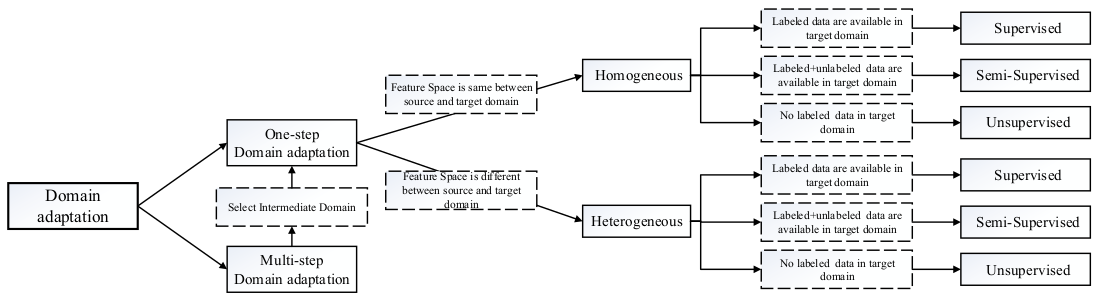
\includegraphics[width=\textwidth]{../images/overview_DA_settings.png}
	\caption{overview of different settings of domain adaptation}
	\label{fig:overview_DA_settings}
\end{figure}


\end{document}